%%%%%%%%%%%%%%%%%%%%%%%%%%%%%%%%%%%%%%%%%
% Jacobs Landscape Poster
% LaTeX Template
% Version 1.0 (29/03/13)
%
% Created by:
% Computational Physics and Biophysics Group, Jacobs University
% https://teamwork.jacobs-university.de:8443/confluence/display/CoPandBiG/LaTeX+Poster
% 
% Further modified by:
% Nathaniel Johnston (nathaniel@njohnston.ca)
%
% Modified further still by:
% Abraham Nunes (nunes <at> dal <dot> ca)
%
% License:
% CC BY-NC-SA 3.0 (http://creativecommons.org/licenses/by-nc-sa/3.0/)
%
%%%%%%%%%%%%%%%%%%%%%%%%%%%%%%%%%%%%%%%%%

%----------------------------------------------------------------------------------------
%	PACKAGES AND OTHER DOCUMENT CONFIGURATIONS
%----------------------------------------------------------------------------------------

\documentclass[final]{beamer}
\usepackage[scale=1.20]{beamerposter}					% Use the beamerposter package for laying out the poster
\usetheme{confposter}									% Use the confposter theme supplied with this template

\setbeamercolor{block title}{fg=black,bg=white}			% Colors of the block titles
\setbeamercolor{block body}{fg=black,bg=white}			% Colors of the body of blocks
\setbeamercolor{block alerted title}{fg=white,bg=black}	% Colors of the highlighted block titles
\setbeamercolor{block alerted body}{fg=black,bg=white}	% Colors of the body of highlighted blocks
% Many more colors are available for use in beamerthemeconfposter.sty

%-----------------------------------------------------------
% Define the column widths and overall poster size
% To set effective sepwid, onecolwid and twocolwid values, first choose how many columns you want and how much separation you want between columns
% In this template, the separation width chosen is 0.024 of the paper width and a 4-column layout
% onecolwid should therefore be (1-(# of columns+1)*sepwid)/# of columns e.g. (1-(4+1)*0.024)/4 = 0.22
% Set twocolwid to be (2*onecolwid)+sepwid = 0.464
% Set threecolwid to be (3*onecolwid)+2*sepwid = 0.708

\newlength{\sepwid}
\newlength{\onecolwid}
\newlength{\twocolwid}
\newlength{\threecolwid}
\setlength{\paperwidth}{48in}				% A0 width: 46.8in
\setlength{\paperheight}{36in}				% A0 height: 33.1in
\setlength{\sepwid}{0.024\paperwidth}		% Separation width (white space) between columns
\setlength{\onecolwid}{0.22\paperwidth}		% Width of one column
\setlength{\twocolwid}{0.464\paperwidth}	% Width of two columns
\setlength{\threecolwid}{0.708\paperwidth}	% Width of three columns
\setlength{\topmargin}{-0.5in}				% Reduce the top margin size
%-----------------------------------------------------------

\usepackage{graphicx}				 	% Required for including images
\usepackage{tikz}						% Used to include a logo
\usepackage{booktabs}					% Top and bottom rules for tables

%----------------------------------------------------------------------------------------
%	TITLE SECTION 
%----------------------------------------------------------------------------------------

\title{Memory allocation: a bottleneck for multithreading.}
\author{Written by \textbf{SID-LAKHDAR Riyane Yacine} (M2 MoSIG: ENSIMAG / UJF)}

\institute{Directed by \textbf{KRAKOWIAK Sacha} (LIG, team ERODS)}

\begin{document}

\addtobeamertemplate{headline}{} 
{
\begin{tikzpicture}[remember picture, overlay]
    \node [anchor=north west, inner sep=6cm]  at (current page.north west)
    {
\includegraphics[height=5cm]{logo/logoINP.png}};
    \node [anchor=north east, inner sep=6cm]  at (current page.north east)
    {
\includegraphics[height=5cm]{logo/logoUJF.jpg}};
    \node [anchor=north east, inner sep=6cm]  at (current page.north east)
    {
\includegraphics[height=5cm]{logo/logoLIG.jpg}};
\end{tikzpicture}
}



%----------------------------------------------------------------------------------------

\addtobeamertemplate{block end}{}{\vspace*{3ex}}			% White space under blocks
\addtobeamertemplate{block alerted end}{}{\vspace*{3ex}}	% White space under highlighted (alert) blocks

\setlength{\belowcaptionskip}{3ex}							% White space under figures
\setlength\belowdisplayshortskip{2ex}						% White space under equations

\begin{frame}[t]											% The whole poster is enclosed in one beamer frame

\begin{columns}[t]											% The whole poster consists of three major columns, the second of which is split into two columns twice - the [t] option aligns each column's content to the top

\begin{column}{\sepwid}\end{column}							% Empty spacer column
\begin{column}{\onecolwid}									% The first column

%----------------------------------------------------------------------------------------
%	OBJECTIVES
%----------------------------------------------------------------------------------------

\setbeamercolor{block alerted title}{fg=white,bg=dalgrey}	% Change the alert block title colors
\setbeamercolor{block alerted body}{fg=black,bg=white}		% Change the alert block body colors

\begin{alertblock}{Objectives}
% I think we should still keep an opening sentence (example: the following sentence)
%Most modern operating systems allow hosted applications to run many execution flows concurrently.   However, the environment they provide is not suitable to optimize the efficiency of such applications.\\

% Try to write the objective of your one month internship in a single sentence
The aim of this study is to analyze and to compare the efficiency of different memory allocation strategies.   Our objective is to compare their time and memory performance for a specific lock implementation.


\end{alertblock}

%----------------------------------------------------------------------------------------
%	CONTEXT
%----------------------------------------------------------------------------------------

\begin{block}{Context}
\begin{itemize}
\item \textbf{Complex multi-core processors:} challenge to maintain and localize data despite of the large number of separated memory component.\\
    \begin{figure}
    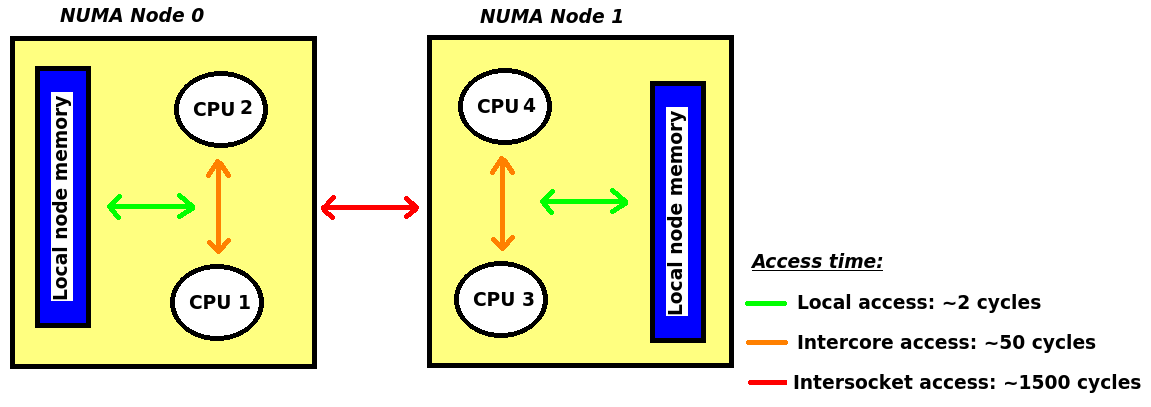
\includegraphics[width=1.0\linewidth]{charts/numaNode.png}
    \caption{Simplified NUMA model (only $\frac{3}{8}$ memory access types)}
    \end{figure}

\item \textbf{Complex concurrent data structure:} Accessed simultaneously by many threads $\Rightarrow$ the sequential memory allocator becomes a bottleneck\\
    \begin{figure}
    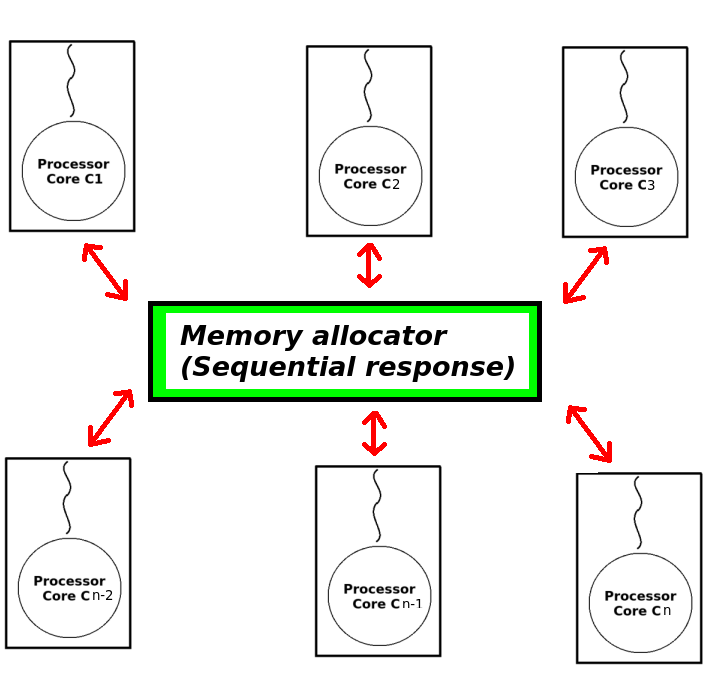
\includegraphics[width=0.9\linewidth]{charts/bottleneck.png}
    \caption{Sequential memory allocator: bottleneck for concurrent thread}
    \end{figure}

\item \textbf{Non-uniform memory access (NUMA):} Non uniform access time may severely harm the performance of highly optimized thread synchronization algorithms.
\end{itemize}


%************* Old objective *************
%Most modern operating systems allow hosted applications to run many execution flows concurrently.   However, the environment they provide is not suitable to optimize the efficiency of such applications.\\

%In this paper we will consider one major component of an operating system: the memory allocator.   This software is sequential.  Thus when different threads try to allocate memory at the same time, they lose the advantages of parallel execution by waiting for the shared allocator.\\

%Our objective is to propose operating system designs to suite the multithreading paradigm.   To do so, we have considered two kind of approaches.\\
%First the software approach, including a new architecture of the memory allocator, or a new architecture for the managed memory.\\
%Second, the hardware approach where we have tried to increase the space locality between each thread`s processor and the memory spans it manages.

%************* End Old objective *************


%With the rise of many-core processors, concurrent programs have increased the efficiency of existing algorithms by simply splitting them tasks over different processors at the same time.   The aim of such a strategy is to improve the execution time of this algorithms by the number of processor.   However this threshold is way of the mark.   The efficiency gain of a parallel execution is limited by hardware and software issues, most importantly including memory allocation.



%This memory allocation strategy is still a standard among the operating system industry. However, different other strategies have been proposed to improve the efficiency of multithreaded applications.    Thus, first of all, we will study the software and hardware interest of some of the most famous and efficient existing allocation strategies.\\

%Second, in order to quantify the efficiency of these strategies, we will design an environment and a set of realistic tests to stress allocators that implement them.   Thanks to this set of custom tests, we want to quantify the efficiency of these strategies and compare them among different situations.\\

%Finally, thanks to the two previous part, we will pick the one (or a mix of multiple) allocation strategy that fits the best to a custom lock implementation.   We will check that the efficiency properties of this lock, computed using a non realistic memory allocation strategy, stay available with the picked strategy.

\end{block}

%----------------------------------------------------------------------------------------

\end{column} % End of the first column

\begin{column}{\sepwid}\end{column}			% Empty spacer column
\begin{column}{\twocolwid}					% Begin a column which is two columns wide (column 2)
\begin{columns}[t,totalwidth=\twocolwid]	% Split up the two columns wide column
\begin{column}{\onecolwid}\vspace{-.6in}	% The first column within column 2 (column 2.1)

%----------------------------------------------------------------------------------------
%	HARDWARE ISSUES
%----------------------------------------------------------------------------------------

\begin{block}{Hardware issues}

\begin{figure}
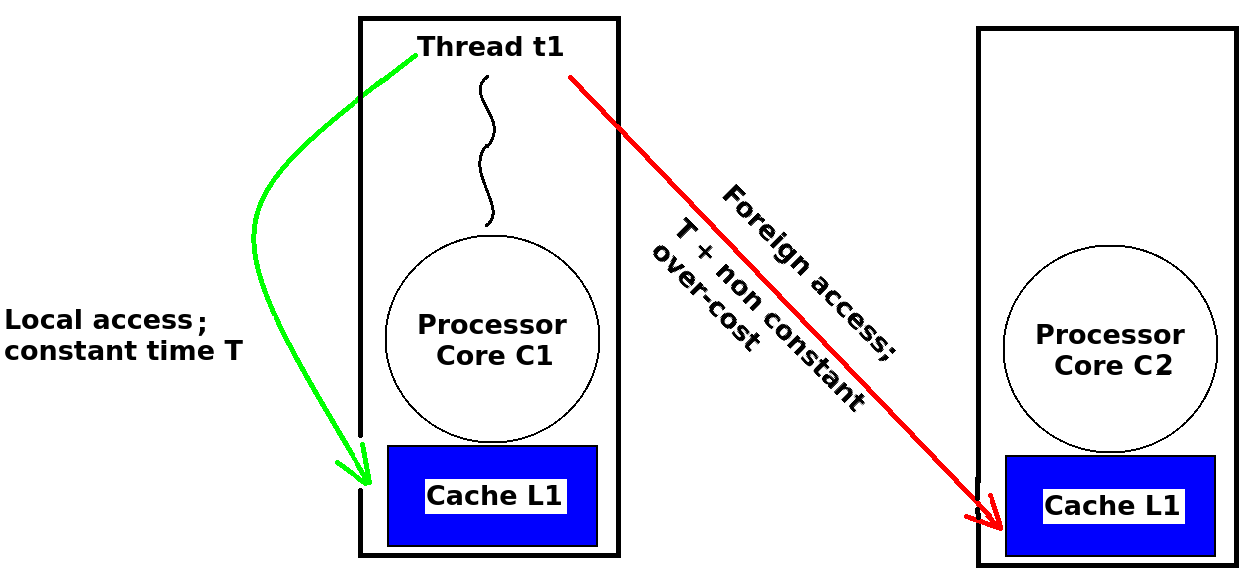
\includegraphics[width=1.0\linewidth]{charts/locality.png}
\caption{Core locality}
\end{figure}

\begin{itemize}
\item \textbf{Cache and memory coherence:} over-cost due to synchronization of separated hardware elements
\item \textbf{Foreign cache access:} client-server request model (or Remote Memory References).
\end{itemize}


\end{block}

%----------------------------------------------------------------------------------------

\end{column} % End of column 2.1

\begin{column}{\onecolwid}\vspace{-.6in} % The second column within column 2 (column 2.2)

%----------------------------------------------------------------------------------------
%	GLOBAL ARCHITECTURE
%----------------------------------------------------------------------------------------

\begin{block}{Global architecture}

\begin{itemize}
	\item Improve thread locality (1 buffer per core)
    \item Decrease synchronization for allocation and memory access (Treiber stack designed to need no synchronization between any core)
\end{itemize}

\begin{figure}
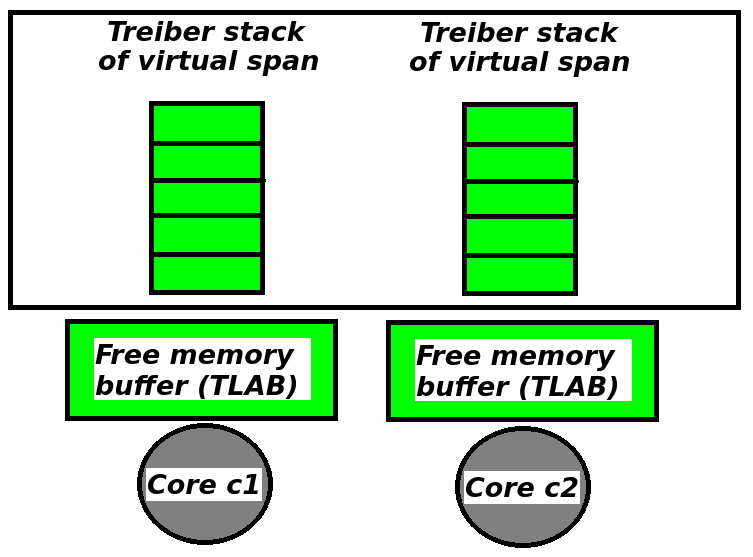
\includegraphics[width=0.8\linewidth]{charts/globalArchitecture.png}
\caption{Free memory pool: shared by all the cores}
\end{figure}

\end{block}

%----------------------------------------------------------------------------------------

\end{column} % End of column 2.2

\end{columns} % End of the split of column 2 - any content after this will now take up 2 columns width

%----------------------------------------------------------------------------------------
%	DESIGNED TEST ENVIRONMENT
%----------------------------------------------------------------------------------------

\setbeamercolor{block alerted title}{fg=black,bg=dalgold} % Change the alert block title colors
\setbeamercolor{block alerted body}{fg=black,bg=white} % Change the alert block body colors

\begin{alertblock}{Designed test environment}
\begin{minipage}{0.4\textwidth}
	\textbf{Interest of the environment}
  \begin{itemize}
		\item The memory allocation is a complex process that involves many other components of the system (hardware and software).
        \item Difficult to test the allocator without being influenced by the performances of the other parts
  \end{itemize}
\end{minipage}
\hspace{0.1\textwidth}
\begin{minipage}{0.4\textwidth}
	\textbf{Formal definition}
  \begin{itemize}
      \item No more threads than cores:
      \item Each thread always run on the same core
  \end{itemize}
\end{minipage}

\end{alertblock} 

%----------------------------------------------------------------------------------------

\begin{columns}[t,totalwidth=\twocolwid] % Split up the two columns wide column again

\begin{column}{\onecolwid} % The first column within column 2 (column 2.1)

%----------------------------------------------------------------------------------------
%	SOFTWARE ISSUES
%----------------------------------------------------------------------------------------

\begin{block}{Software issues}

\begin{itemize}
\item \textbf{Contention and synchronization over-cost:} The allocator is shared between all threads.
\item \textbf{Context switch cost:} depends on the processor architecture (task state segment) and the data transfer throughput (memory word size).
\item \textbf{Fragmentation and memory blowup}
\item \textbf{False sharing:} Occurs when multiple processors share a word in the same cache line without actually sharing data (useless synchronization over-cost).
\begin{figure}
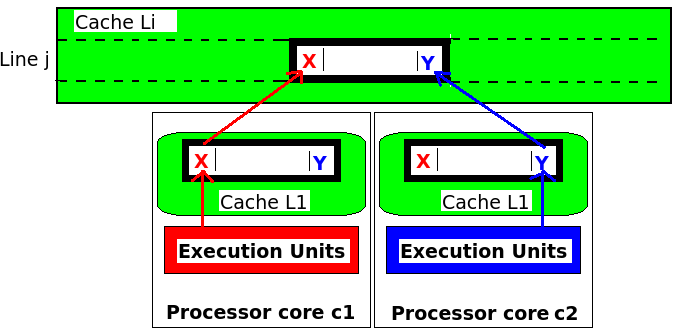
\includegraphics[width=1.0\linewidth]{charts/falseSharing.png}
\caption{False sharing representation}
%\caption{False sharing representation \footnote{Inspired from the article of BROOK Mohamed, posted September 06, 2014 within the online journal "http://www.programering.com"}}
\end{figure}

\end{itemize}


\end{block}

%----------------------------------------------------------------------------------------

\end{column} % End of column 2.1

\begin{column}{\onecolwid} % The second column within column 2 (column 2.2)

%----------------------------------------------------------------------------------------
%	CORE LOCAL STACK: 
%----------------------------------------------------------------------------------------

\begin{block}{Core local Treiber stack}

\begin{figure}
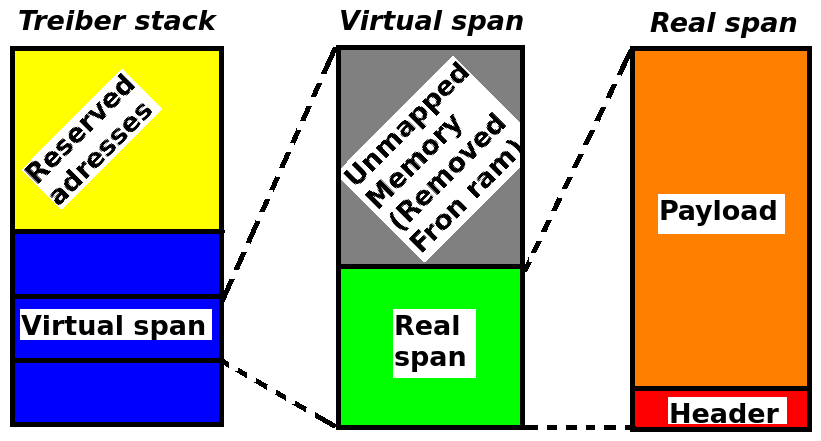
\includegraphics[width=0.8\linewidth]{charts/treiberStack.png}
\caption{Structure and content of a Treiber stack}
\end{figure}

\begin{itemize}
	\item Delegate memory allocation to user program $\Rightarrow$ No system call
    \item Constant size span $\Rightarrow$ no false sharing + no external fragmentation
    \item Treiber stack per core $\Rightarrow$ constant time allocation
\end{itemize}

\end{block}

%----------------------------------------------------------------------------------------

\end{column}						% End of column 2.2
\end{columns}						% End of the split of column 2
\end{column}						% End of the second column
\begin{column}{\sepwid}\end{column}	% Empty spacer column
\begin{column}{\onecolwid}			% The third column

%----------------------------------------------------------------------------------------
%	EXPERIMENTAL RESULTS
%----------------------------------------------------------------------------------------

\begin{block}{Experimental results}
	\begin{itemize}
    	\item Average time improvement of $20 \rightarrow 40$ \% compared to the c standard library
    	\item Average time improvement of $10 \rightarrow 20$ \% compared to existing implementation designed for multithreading
		\item Very different results depending on the environment
	\end{itemize}
\begin{figure}
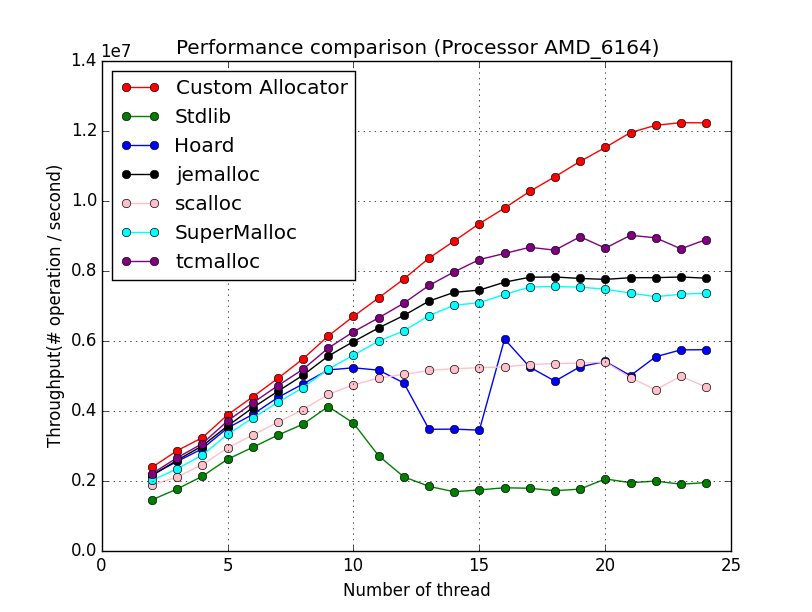
\includegraphics[width=0.8\linewidth]{charts/result.png}
\caption{Average throughput comparison between memory allocators}
\end{figure}

\end{block}

%----------------------------------------------------------------------------------------
%	CONCLUSION
%----------------------------------------------------------------------------------------

\setbeamercolor{block alerted title}{fg=white,bg=black}	% Change the alert block title colors
\setbeamercolor{block alerted body}{fg=black,bg=white}		% Change the alert block body colors

\begin{alertblock}{Conclusion}

During this study, we have
	\begin{itemize}
		\item Designed and explored memory allocation strategies
        \item Highlighted the existing designs that limit the performances of multithreaded applications 
     \end{itemize}
We have also implemented an allocator with
	\begin{itemize}
     	\item Interesting time and memory gain compared to the existing ones
        \item Stable performance (interesting for research purposes)
	\end{itemize}
\end{alertblock}

%----------------------------------------------------------------------------------------
%	REFERENCES
%----------------------------------------------------------------------------------------

\begin{block}{References}



\nocite{*} % Insert publications even if they are not cited in the poster
\small{\bibliographystyle{unsrt}
\bibliography{bibliography.bib}\vspace{0.75in}}

\end{block}

%----------------------------------------------------------------------------------------

\end{column}	% End of the third column
\end{columns}	% End of all the columns in the poster
\end{frame}		% End of the enclosing frame



\end{document}
